\documentclass{article}

\usepackage{color}
\usepackage{graphicx}
\usepackage{tabularx}


\usepackage{geometry}
 \geometry{
 top=20mm,
 bottom=20mm,
 }


\title{Document de pr\'esentation}
\author{Justal Kevin}
\date{26/09/2015}
\renewcommand{\contentsname}{Table des matieres} 
 
\newcommand\invisiblesection[1]{%
  \refstepcounter{section}%
  \addcontentsline{toc}{section}{\protect\numberline{\thesection}#1}%
  \sectionmark{#1}} 
 
\begin{document}

\begin{center}
\textbf{\Huge{LES ANIMAUX}}
\line(1,0){300}\\
DOSSIER DE CONCEPTION\\
\vspace{3cm}
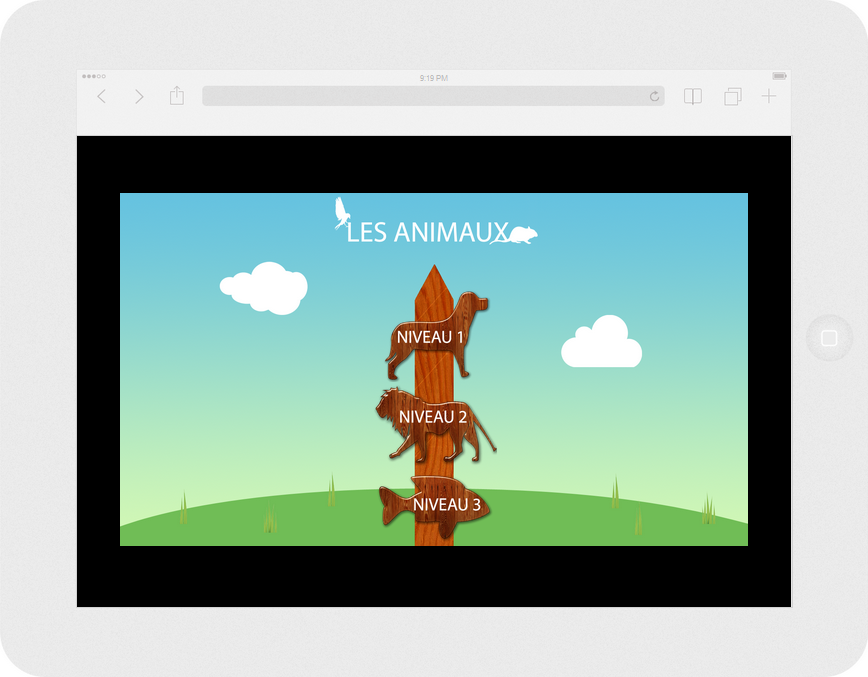
\includegraphics[width=0.8\textwidth]{tablette}\\
\vspace{3cm}
\textbf{Justal Kevin - \color{blue}{\underline{justal@polytech.unice.fr}} \color{black}{- SI5 - IHM}}\\
\textbf{Justal Kevin - \color{blue}{\underline{justal@polytech.unice.fr}} \color{black}{- SI5 - IHM}}\\
\textbf{Justal Kevin - \color{blue}{\underline{justal@polytech.unice.fr}} \color{black}{- SI5 - IHM}}\\
\vspace{4cm}
\textbf{Encadrant :}\\
\textbf{Jean-Paul Stromboni - \color{blue}{\underline{strombon@polytech.unice.fr}}}
\end{center}

\newpage
\tableofcontents

\newpage

\section{Pr\'esentiation de l'application}
\hspace*{0.6cm}Les jeux accessibles sont un bon moyen d'aid\'e le d\'eveloppement intellectuel et psychologique des enfants handicap\'es. C'est pour cela que nous avons décidé de produire un jeu le plus simple possible faisant travailler l'intelligence logico-math\'ematique et corporelle kinesth\'esique des enfants. Le jeu confronte les enfants à plusieurs images d'animaux et des cases o\^u chaque animal peut \^etre rang\'e. Les enfants devront donc associer des animaux ayant le m\^eme nombre de pattes, le m\^eme type d'habitation ou encore suivant la cat\'egorie de l'animal (domestiques, de la ferme, sauvages).
\section{Struction de l'application}

La structure g\'enerale de notre application sera la suivante :
\vspace{0.5cm}\\
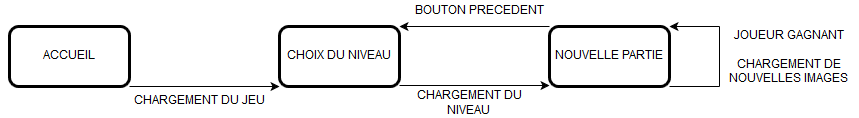
\includegraphics[width=\textwidth]{plan}
\vspace{0.5cm}\\
\hspace*{0.6cm}La structure est volontairement simple afin que toutes personnes puissent prendre le jeu en main sans aucune indication.\\
Une fois la page d'accueil charg\'e, le choix des diff\`erents niveaux s'affiche. Lorsque l'utilisateur clique sur l'une des options, le jeu lance le niveau selectionn\'e.\\
Si l'utilisateur d\'ecide d'arr\^eter le jeu ou de changer de niveau, il peut alors revenir au menu du depart en cliquant sur le bouton "retour". 

\section{Storyboard}
\hspace*{0.6cm}Le jeu dispose de quatre sc\`enes cl\'es qui \`a elles seules suffisent pour d\'ecrire le jeu entier. Dans chaque section du jeu, nous verrons en d\'etails les objectifs et les accomplissements que l'on attend du joueur. 
\subsection{Ecran d'accueil}
\vspace{0.5cm}
\begin{center}
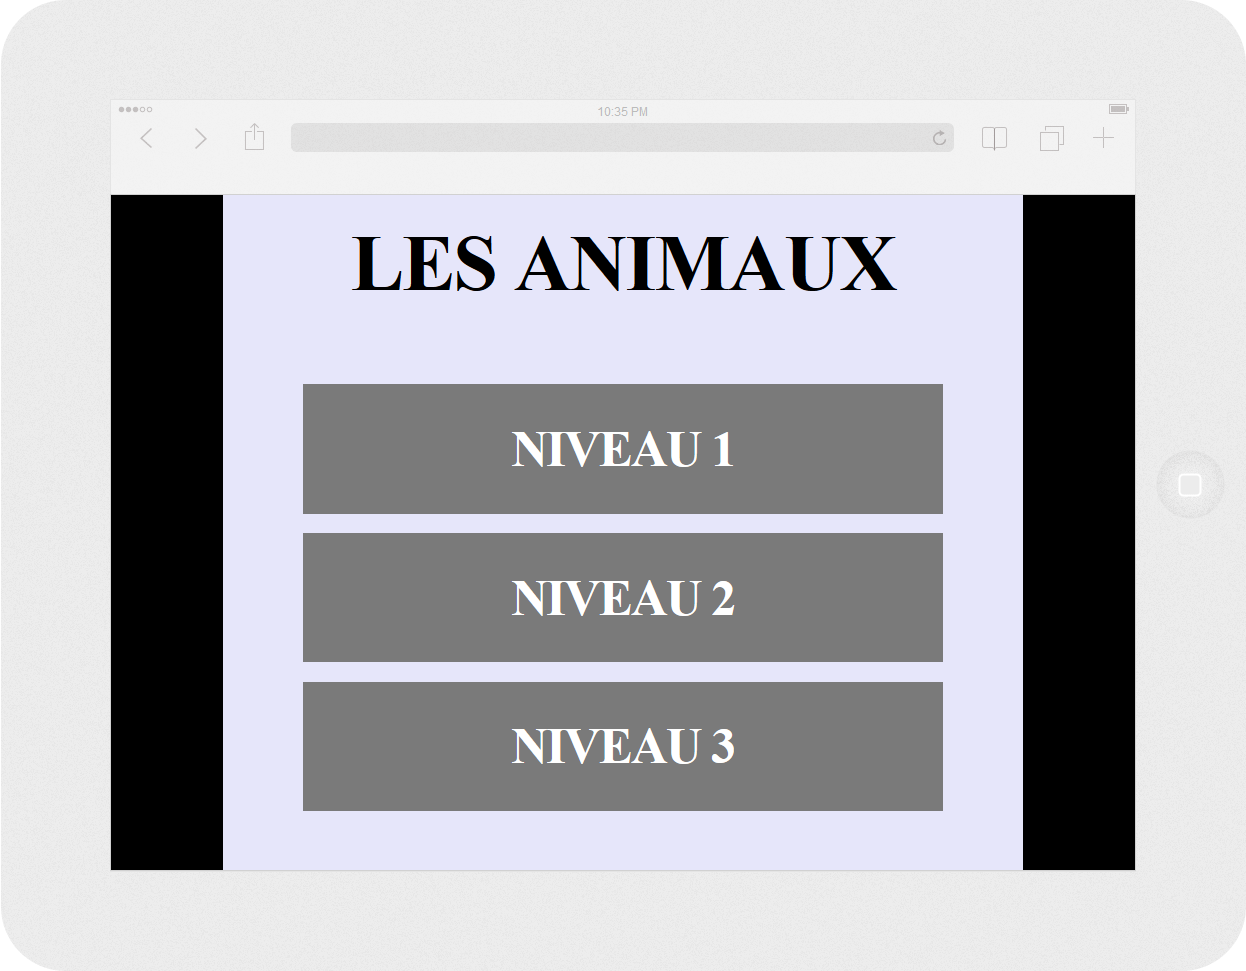
\includegraphics[width=0.6\textwidth]{page1}
\end{center}
\vspace{0.5cm}
\hspace*{0.6cm}Le menu est tr\`es simple, \'epur\'e de tout contenu additionnel inutile. Le texte est \'ecrit tr\`es gros au cas o\`u l'enfant aurait un handicap au niveau de la vue. De m\^eme pour \'eviter que l'enfant n'ouvre pas les options du navigateur au cas o\`u le jeu \'etait lanc\'e sur un ordinateur, le clic droit a \'et\'e d\'esactiv\'e.Le cursor a aussi \'et\'e modifi\'e, il est beaucoup plus grand que la normal si l'enfant aurait un handicap au niveau e la vue.
\vspace{0.5cm}\\
\hspace*{0.6cm}Sinon concernant le menu, il y a le minimum d'animation pour que le joueur puisse s'y retrouver. Lorsque le joueur passe la souris sur les diff\`erents niveaux, ces derniers se surlignent et grossissent l\'eg\`erement.
\subsection{Niveau 1 - Trier par cat\'egories}
\vspace{0.5cm}
\begin{center}
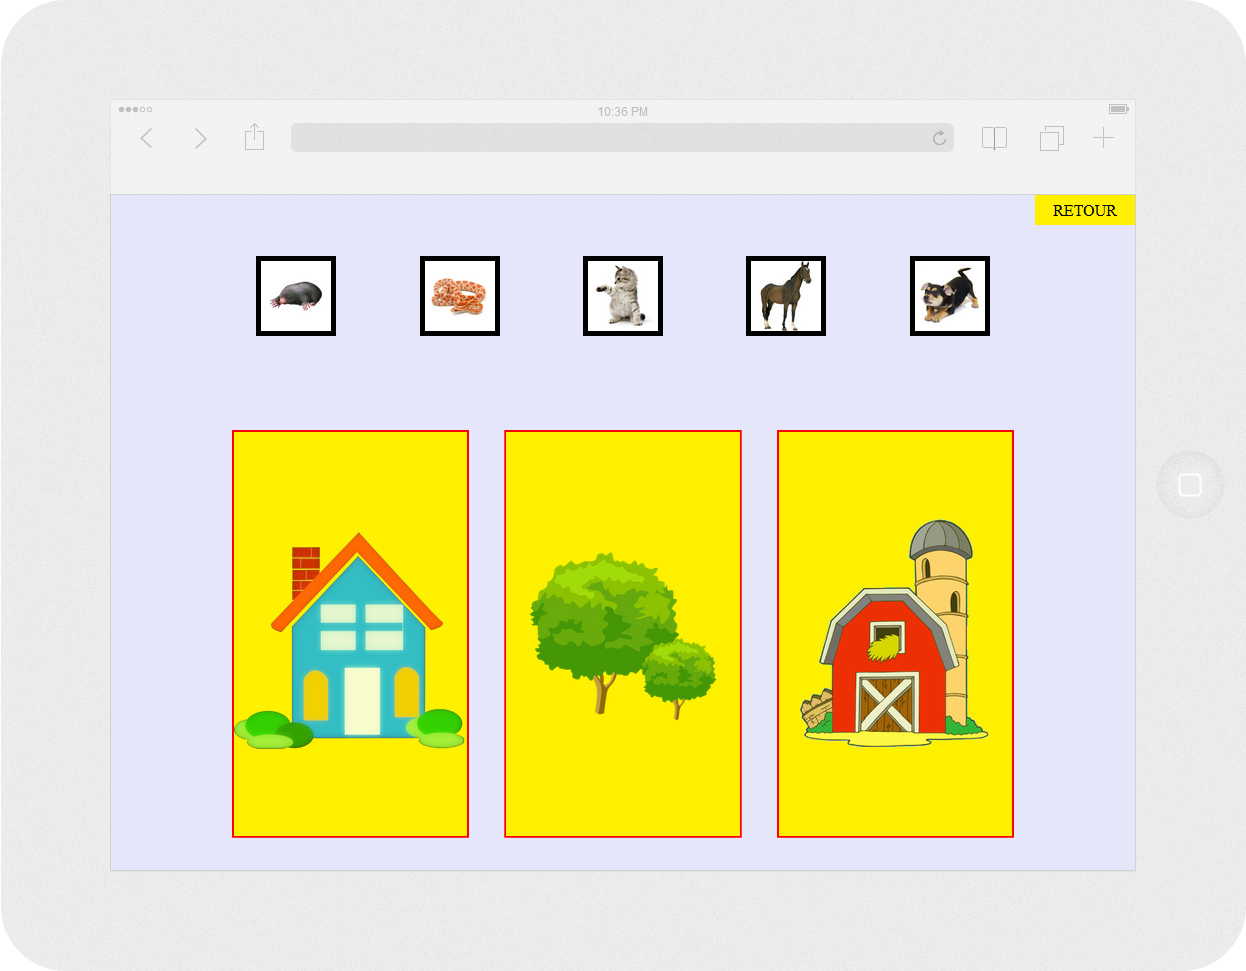
\includegraphics[width=0.6\textwidth]{page2}
\end{center}
\vspace{0.5cm}
\hspace*{0.6cm}Comme l'ensemble du jeu, les niveaux sont eux aussi simplifi\'e au maximum.
Le premier niveau consiste \`a associer les animaux affich\'es dans leurs cat\'egories respectives. Prenons un exemple, un chat ira dans la cat\'egorie domestique. On glisse alors l'image du chat sur la case jaune avec une maison. En cas de bonne r\'eponse, l'image reste dans la case pr\'evue. En cas de mauvaise r\'eponse, l'image retourne \`a son emplacement d'origine.
\subsection{Niveau 2 - Trier par nombre de pattes}
\vspace{0.5cm}
\begin{center}
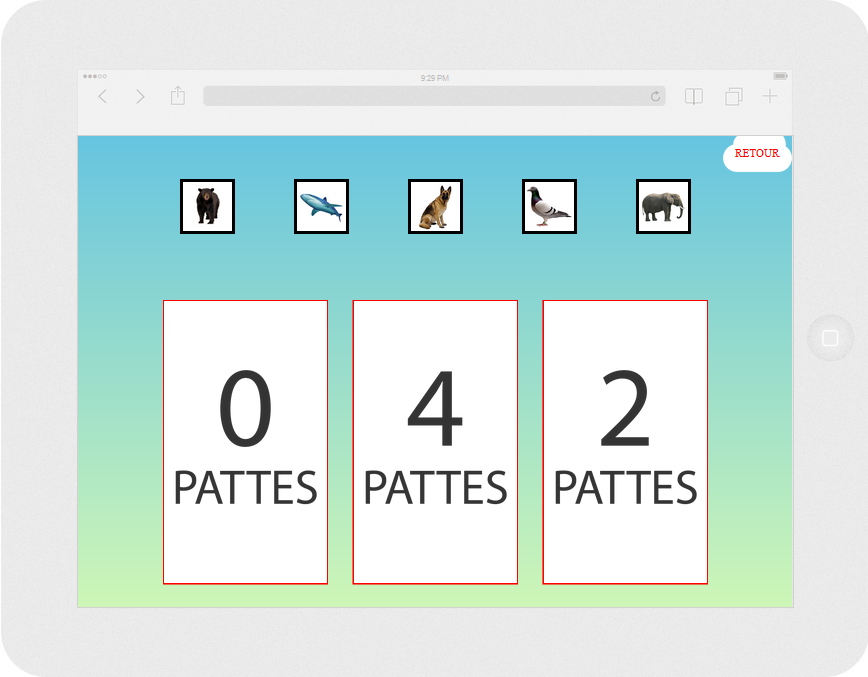
\includegraphics[width=0.6\textwidth]{page3}
\end{center}
\vspace{0.5cm}
\hspace*{0.6cm}Le niveau 2 est semblable au premier dans sa structure mais le jeu est plus difficile que le niveau 1. Dans ce niveau, le joueur doit trier les animaux par nombre de pattes. Par exemple, la case jaune avec le chien est la case qui regroupe les animaux avec 4 pattes comme le chat.
\subsection{Niveau 3 - Trier par habitation}
\vspace{0.5cm}
\begin{center}
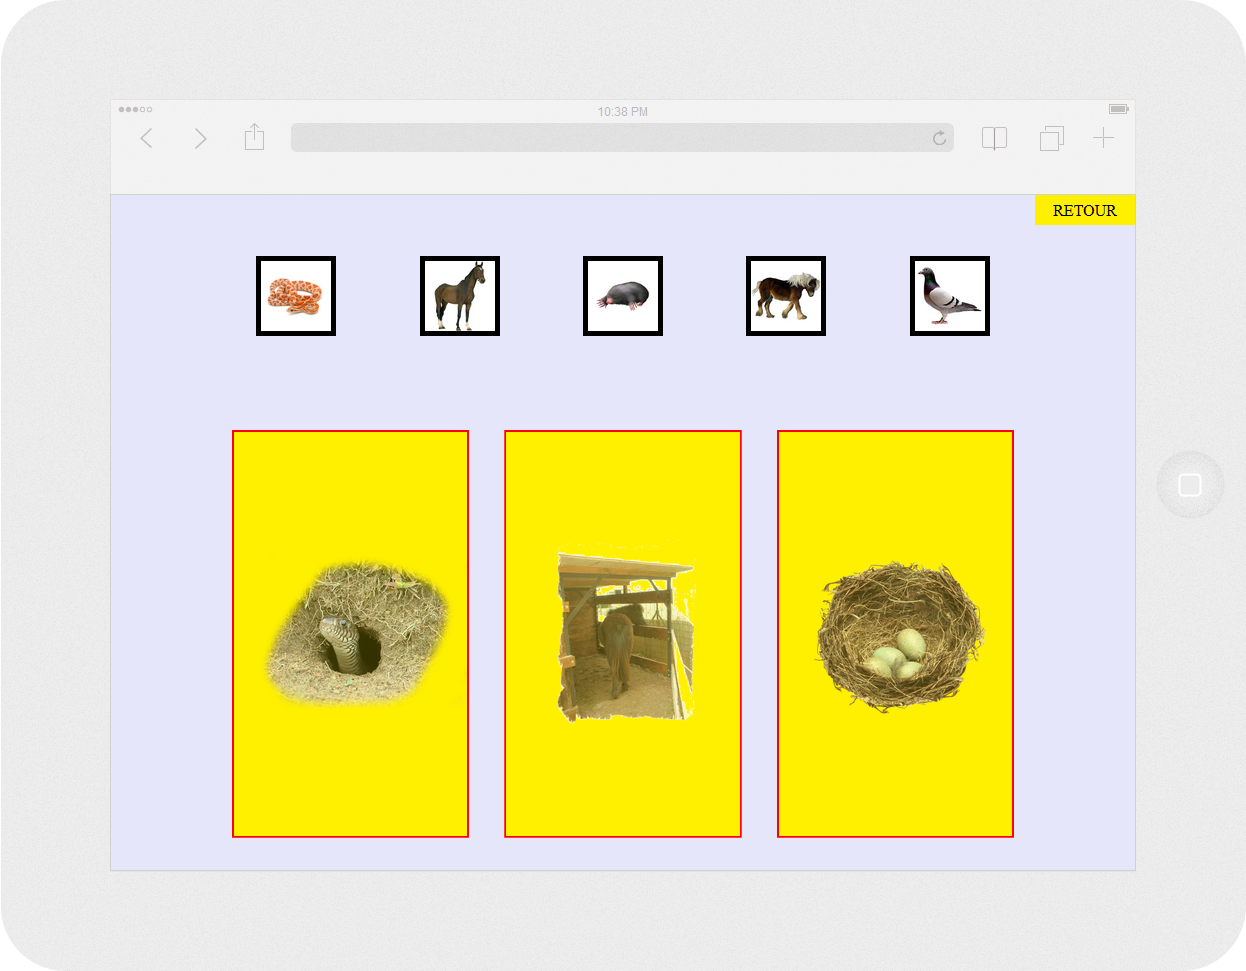
\includegraphics[width=0.6\textwidth]{page4}
\end{center}
\vspace{0.5cm}
\hspace*{0.6cm}Le dernier niveau est le plus difficile de tous. Cependant la structure et le gameplay restent l\`a aussi similaire au deux niveaux pr\'ec\'edent. Seul les associations avec les animaux diff\`erent. Cette fois, les animaux sont tri\'e suivant leurs habitations. Pour continuer avec les exemples, prenons le cheval, ce dernier vit dans une \'ecurie. On d\'eplacera donc l'image du cheval dans la case repr\'esentant l'\'ecurie.
    
\section{Gameplay}

Le jeu est d\'ecompos\'e en deux parties. En haut (zone1 en rouge), vous trouverez les animaux que vous pouvez d\'eplacer et en bas (zone 2 en violet) les zones o\`u vous pouvez les d\'eplacer.
\vspace{0.5cm}\\
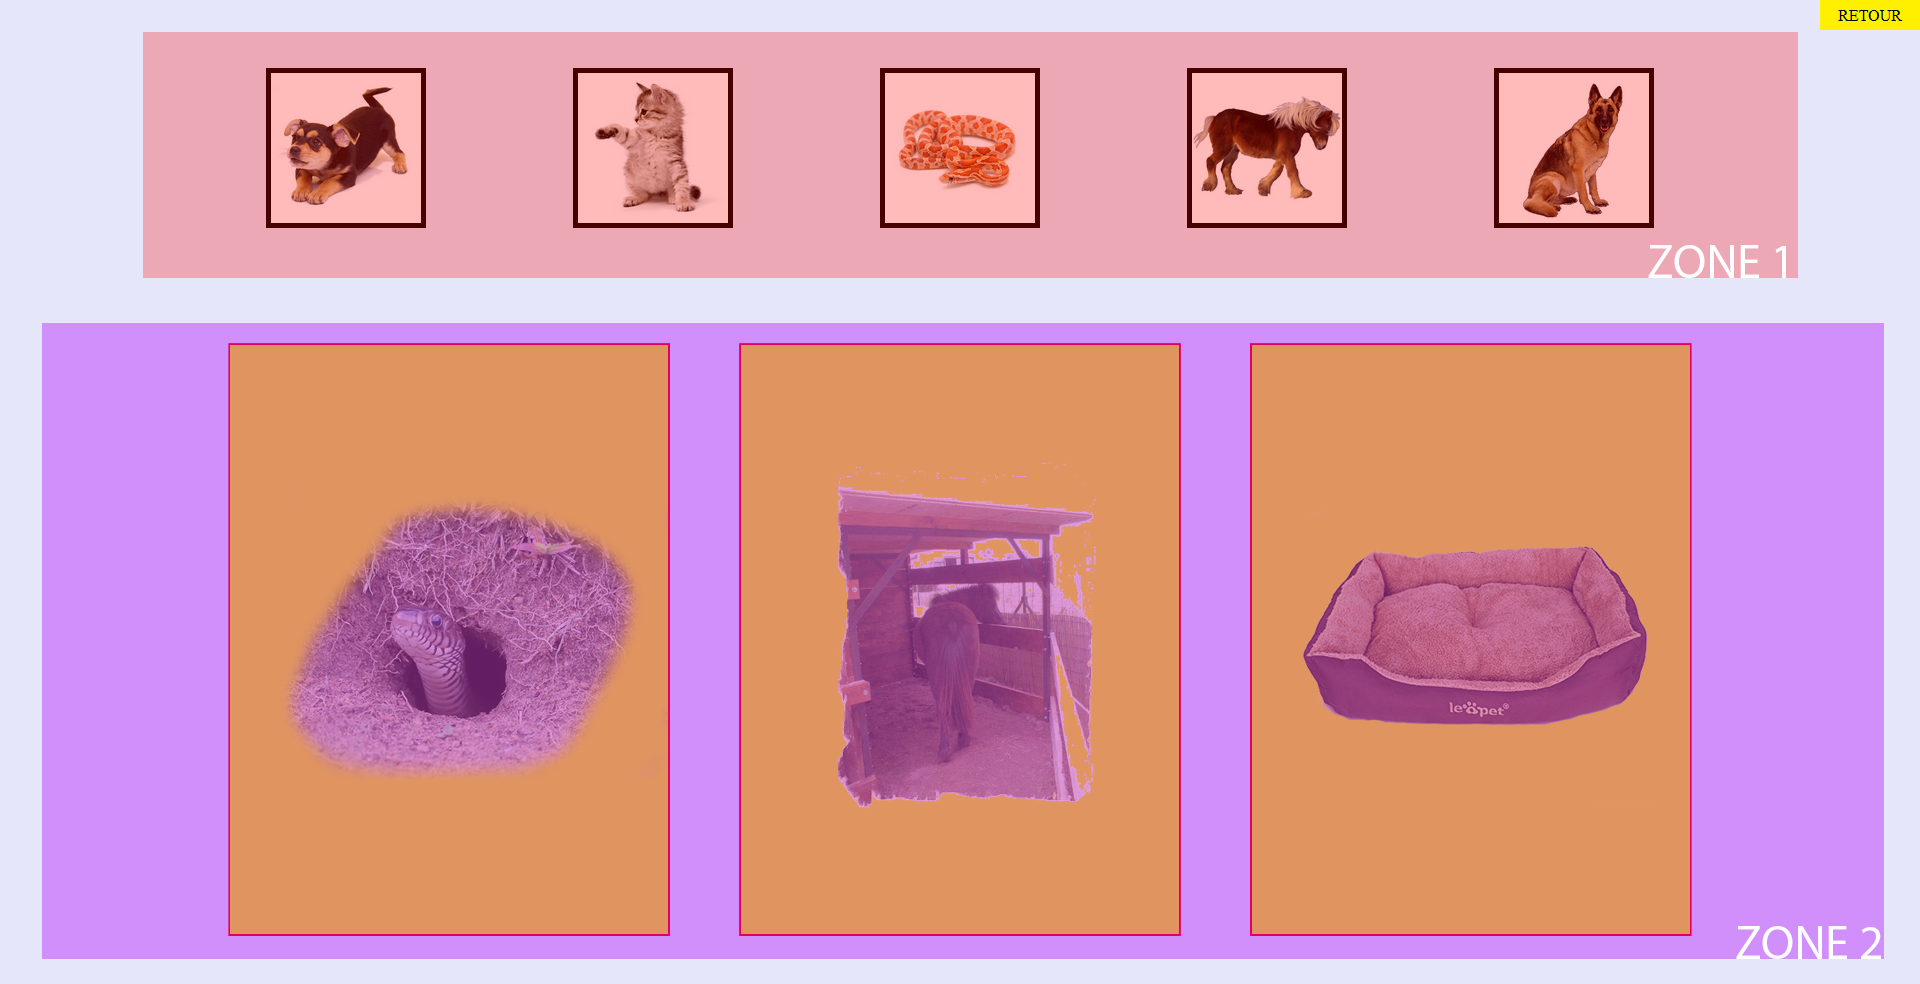
\includegraphics[width=1.0\textwidth]{zone}
\vspace{0.5cm}\\
Le but du jeu est d\'eplacer les animaux de la zone 1 vers la zone 2 en suivant une certaine logique. Reprenons notre exemple pr\'ec\'edent et notons les animaux de la zone 1.\\
\vspace{0.5cm}\\
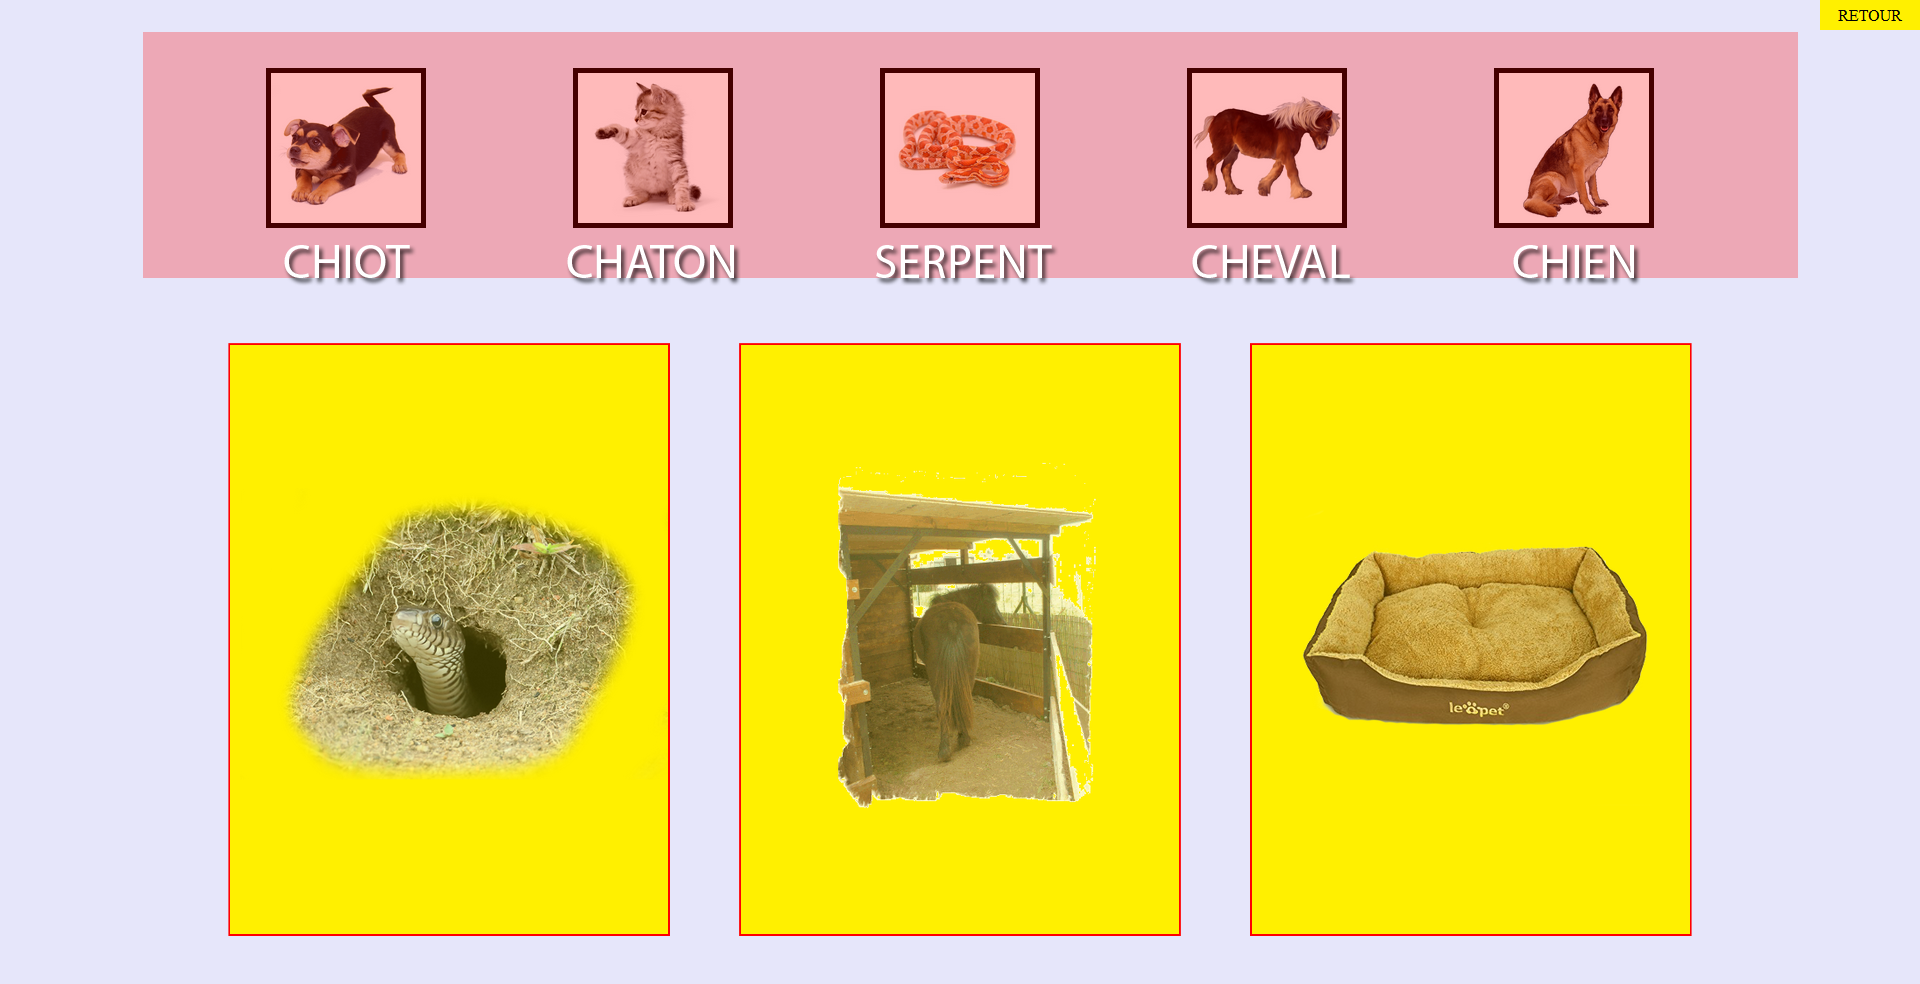
\includegraphics[width=1.0\textwidth]{zone1}
\vspace{0.5cm}\\
Prenons par exemple le cheval, nous allons cliquer dessus et maintenir notre clique tout en d\'epla\c{c}ant la souris.
\vspace{0.5cm}\\
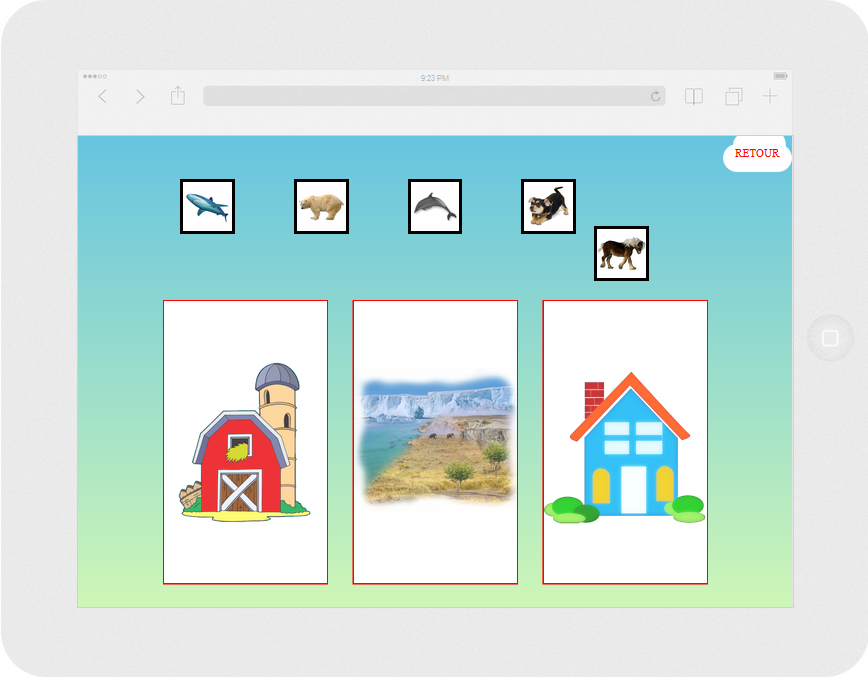
\includegraphics[width=1.0\textwidth]{zone2}
\vspace{0.5cm}\\
Si nous rel\^achons notre clique, l'image du cheval retournera \'a sa place automatiquement. Maintenant, regardons avec attention la zone 2 et d\'ecrivons l\`a aussi les images. 
\vspace{0.5cm}\\
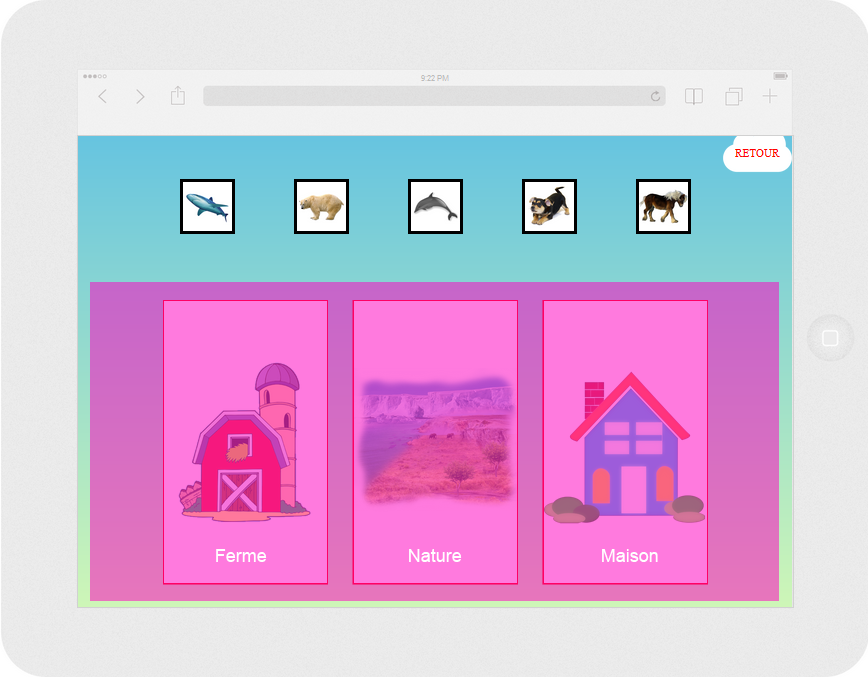
\includegraphics[width=1.0\textwidth]{zone3}
\vspace{0.5cm}\\
Reprenons maintenant notre cheval et d\'epla\c{c}ont le dans la zone qui lui correspond (l'écurie). L'image se fixera alors \`a la zone et vous ne pourrez plus y toucher. Vous avez la bonne r\'eponse !
\vspace{0.5cm}\\
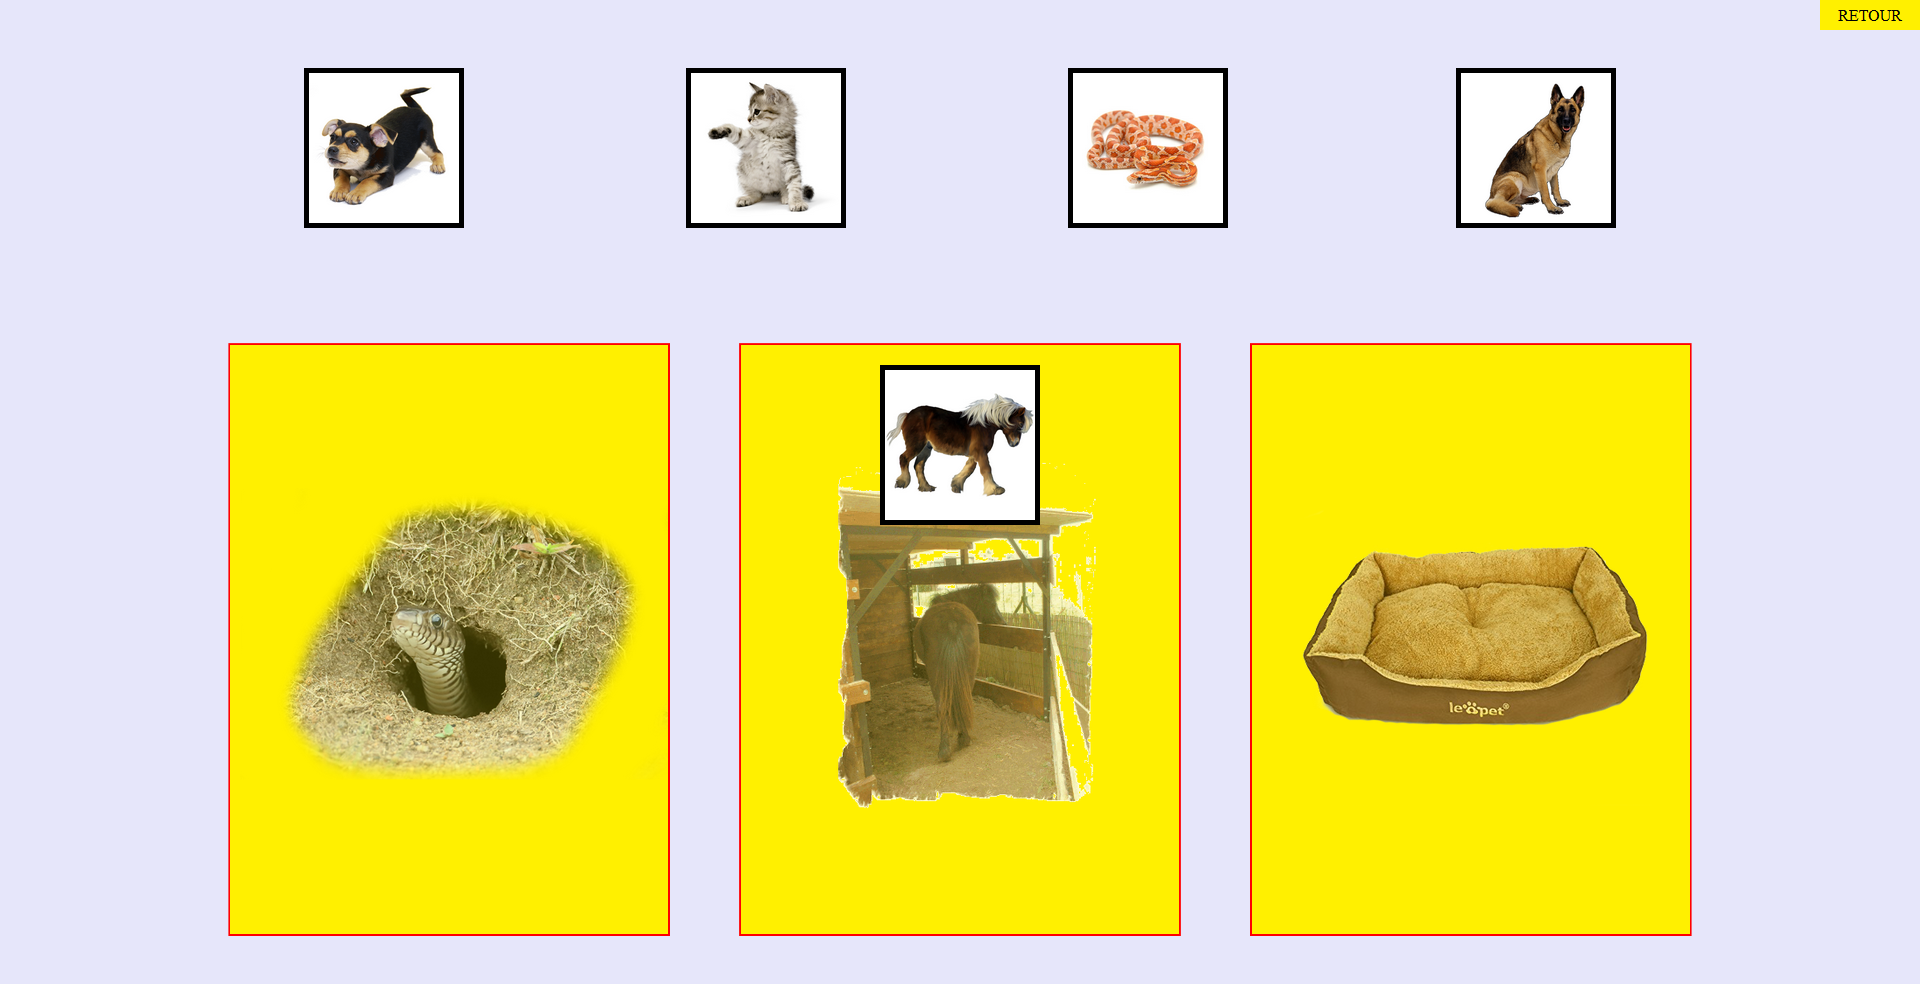
\includegraphics[width=1.0\textwidth]{zone4}
\vspace{0.5cm}\\
Maintenant effectuons cette m\^eme op\'eration pour chaque image restante dans la zone 1. Allez, encore un petit effort, nous y somme presque.
\vspace{0.5cm}\\
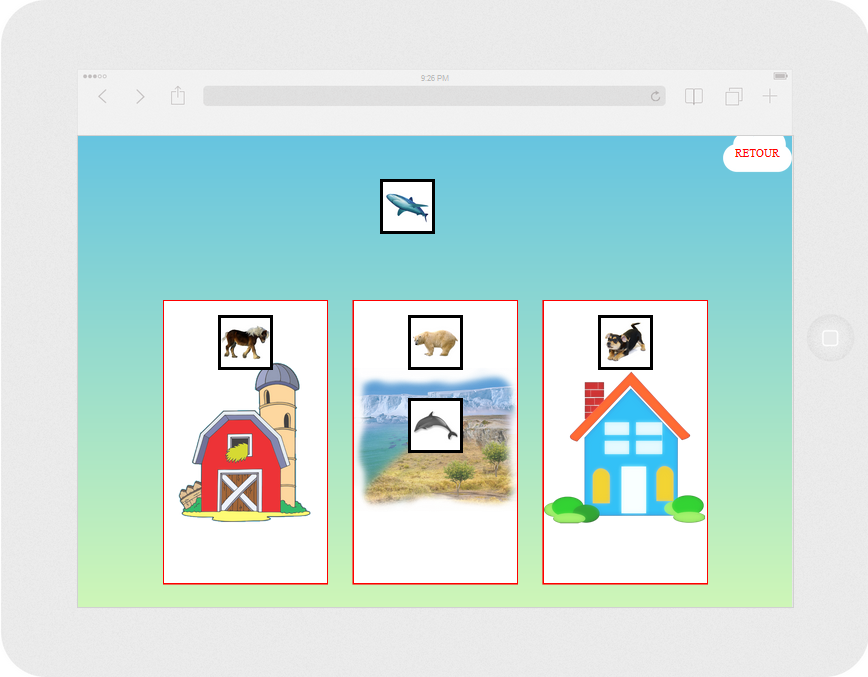
\includegraphics[width=1.0\textwidth]{zone5}
\vspace{0.5cm}\\
Si vous r\'epondez correctement en pla\c{c}ant l'integralit\'e des images, un message vous disant "Bravo" s'affiche alors pour vous f\'eliciter.
\vspace{0.5cm}\\
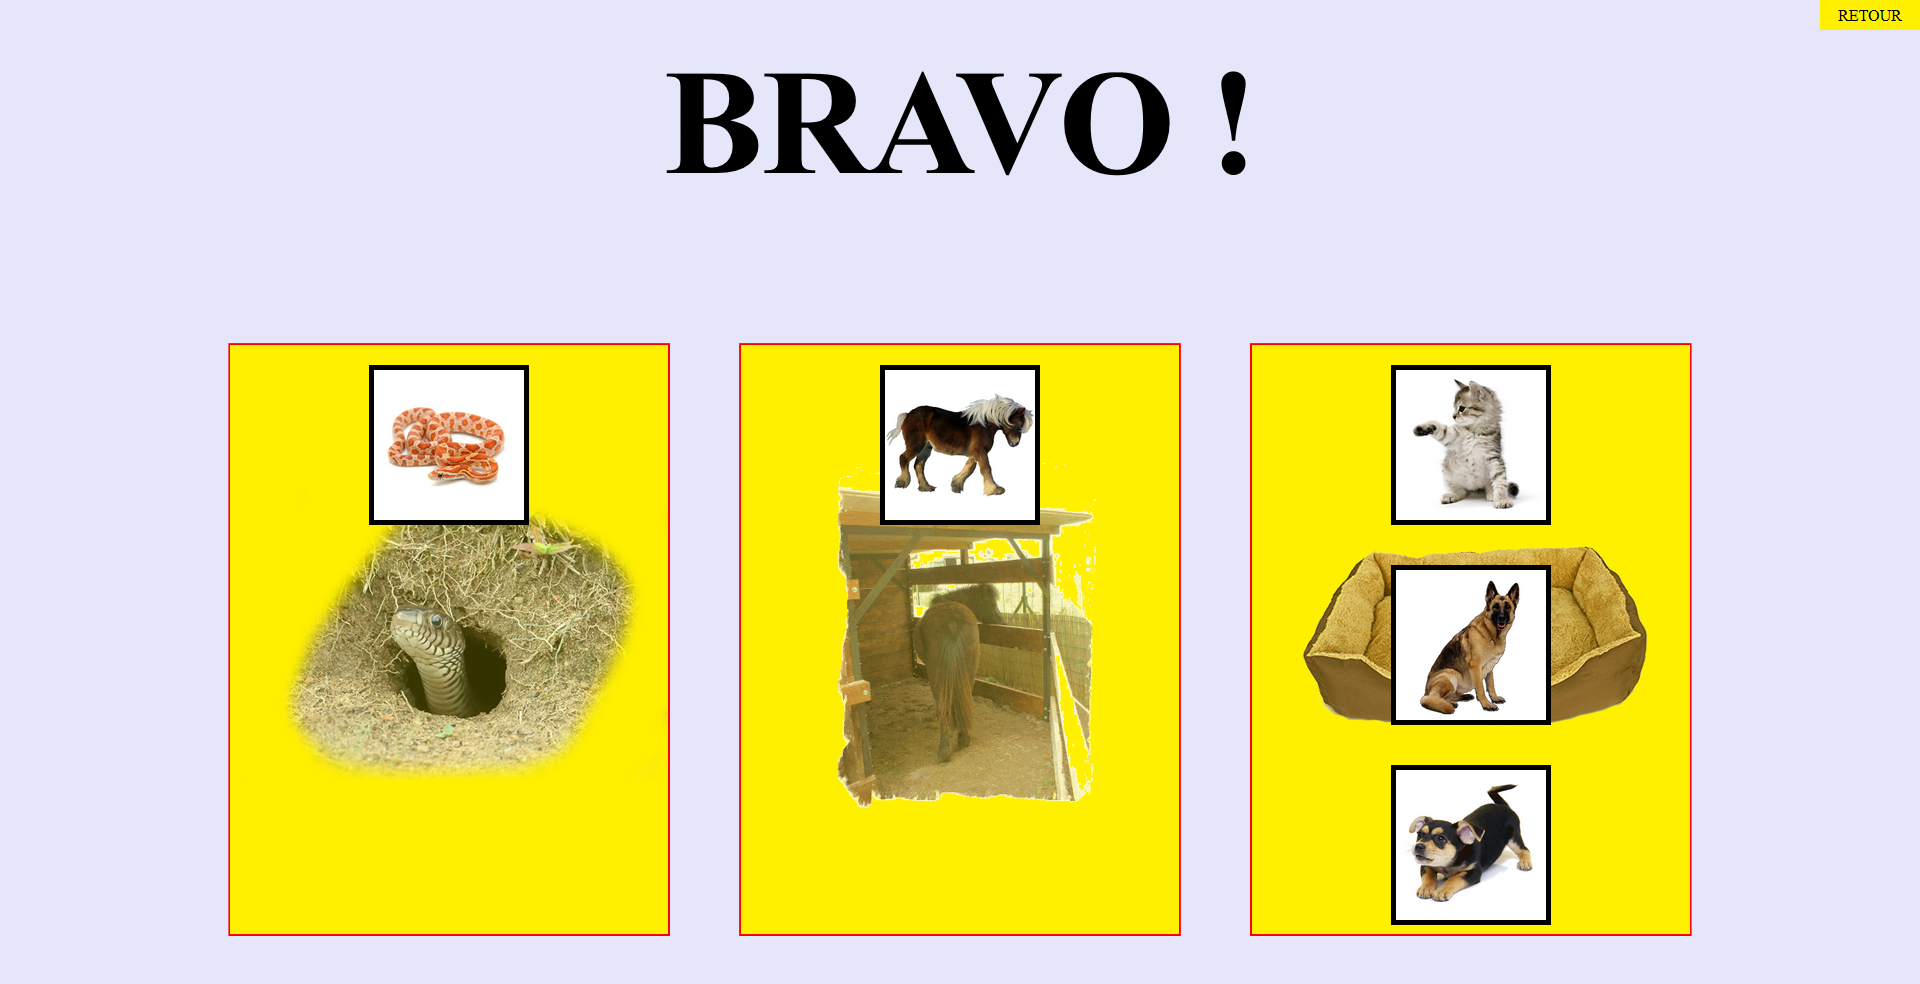
\includegraphics[width=1.0\textwidth]{zone6}
\vspace{0.5cm}\\
Puis une nouvelle partie commence avec de nouveaux \'el\'ement dans les deux zones.
\vspace{0.5cm}\\
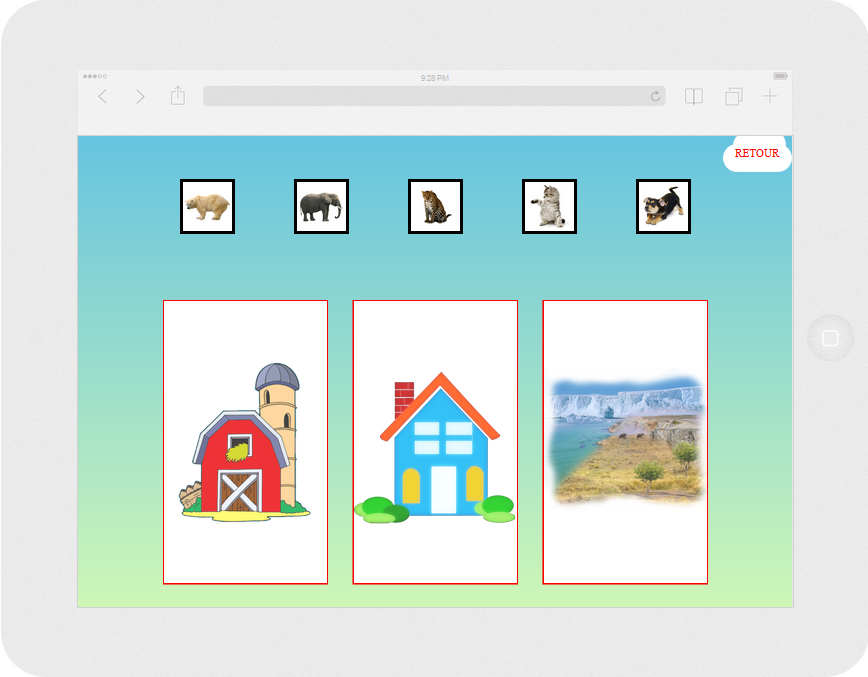
\includegraphics[width=1.0\textwidth]{zone7}
\vspace{0.5cm}\\


\section{Mise en oeuvre - Outils utilis\'es}
\hspace*{0.6cm}Pour le d\'eveloppement, nous allons utiliser l'HTML5, le CSS3 et le JavaScript ainsi qu'une librairie permettant de faciliter le code javascript: JQuery. Le jeu sera compatible sous tous les navigateurs autre que IE, c'est \`a dire : Google Chrome, Mozilla Firefox, Safari, Opera.
Pour les images utilis\'ees dans le jeu, nous utiliserons des images issus d'internet et nous les modifierons avec photoshop pour les rendre les plus simple possible.\\
Pour partager le code efficacement, nous avons utilis\'e GIT.
\section{Planning}

\begin{tabular*}{1.0\textwidth}{@{\extracolsep{\fill}} | c | l | }
  \hline
  & Choix du sujet\\
  & Cr\'eation du dossier de conception\\
  Semaine 1 & Cr\'eation du premier prototype\\
  & \'Ecriture de la documentation\\
  & Test de la version 1.0\hspace*{9.6cm}\\
  \hline
  & Ajout de nouvelles id\'ees\\ 
  Semaine 2  & Am\'elioration du prototype jusqu'\`a la version final\\
  & Test des versions intermediaires\\
  \hline
  Semaine 3  & Test et finalisation graphique\\
  \hline
  & Correctifs des d\'etails\\
  Semaine 4-8 & Ajout de donn\'es\\
  & Tests finaux\\
  \hline
\end{tabular*}

\end{document}